\documentclass[a4paper,12pt]{article}
\setlength{\headheight}{68.803pt}
\addtolength{\topmargin}{-56.803pt}

\usepackage[utf8]{inputenc}
\usepackage[T1]{fontenc}
\usepackage[italian]{babel}
\usepackage{lmodern}
\usepackage{fvextra}
\DefineVerbatimEnvironment{Verbatim}{Verbatim}{
  breaklines=true,
  breakanywhere=true,
  frame=single,
  fontsize=\small
}

% Impostazione dei margini con geometry
\usepackage[
  left=1in,
  right=1in,
  top=3cm,
  bottom=1in
]{geometry}

\usepackage[
    colorlinks=true,
    linkcolor=black,
    urlcolor=blue,
    citecolor=blue,
    pdfborder={0 0 0},
    pdfauthor={Massimo Mantineo},
    pdftitle={Progetto 1: Segmentazione clienti e Churn Prediction},
    pdfsubject={Laboratorio di Intelligenza Artificiale},
]{hyperref}

\usepackage{graphicx}
\usepackage{listings}
\usepackage{xcolor}
\usepackage{amsmath, amssymb}
\usepackage{fancyhdr}
\usepackage{setspace}
\usepackage{pgfplots}
\pgfplotsset{compat=1.17}
\usepackage{booktabs}
\usepackage{float}
\usepackage{enumitem}
\usepackage{caption}
\usepackage{microtype}
\usepackage{titlesec}

\setlength{\footskip}{50pt}

% Impostazioni per i listing del codice Python
\lstdefinestyle{pythonstyle}{
    language=Python,
    basicstyle=\ttfamily\small,
    numbers=left,
    numberstyle=\tiny,
    stepnumber=1,
    numbersep=5pt,
    backgroundcolor=\color{white},
    showspaces=false,
    showstringspaces=false,
    showtabs=false,
    frame=single,
    tabsize=4,
    captionpos=b,
    breaklines=true,
    breakatwhitespace=true,
    keywordstyle=\color{blue}\bfseries,
    commentstyle=\color{green!50!black},
    stringstyle=\color{red},
}
\lstset{style=pythonstyle}

% Impostazione di fancyhdr per header e footer
\pagestyle{fancy}
\fancyhf{}

\fancyhead[L]{%
  \parbox[b]{0.45\textwidth}{%
    \small
    Student Name: Massimo Mantineo\\
    Student ID: 541924
    \vspace{8pt}
  }%
}
\fancyhead[C]{%
  \parbox[b]{0.2\textwidth}{%
    \centering
    \normalsize \bfseries
    Lab IA\\
    25/26
    \vspace{8pt}
  }%
}
\fancyhead[R]{%
  \parbox[b]{0.35\textwidth}{%
    \flushright
    \includegraphics[width=3.5cm]{\detokenize{logo_unime_orizontale.png}}
    \vspace{8pt}
  }%
}

\renewcommand{\contentsname}{Indice}

\begin{document}

% Pagina di copertina
\begin{titlepage}
    \thispagestyle{empty}
    \centering
    \vspace*{1cm}
    \includegraphics[width=6cm]{\detokenize{logo_unime_orizontale.png}}\par\vspace{1cm}
    \vspace{2cm}
    {\Large \textbf{Università degli Studi di Messina}\par}
    {\large Dipartimento MIFT - Corso di Laurea Triennale in Informatica (L-31)\par}
    \vspace*{1.5cm}
    {\large Laboratorio di Intelligenza Artificiale\par}
    \vspace{1.5cm}
    {\Large \textbf{PROGETTO 1:}\\
    Segmentazione Clienti e Churn Prediction\par}
    \vspace{2.5cm}
    {\large Massimo Mantineo \par}
    {\large Matricola: 541924 \par}
    \vfill
    {\large Messina, A.A. 2025/2026 \par}
\end{titlepage}

\clearpage
\pagestyle{fancy}
\tableofcontents
\newpage

\begin{abstract}
In questo progetto ho studiato come unire il clustering (apprendimento non supervisionato) e la classificazione (apprendimento supervisionato) per analizzare il comportamento dei clienti di una compagnia telefonica (usando il dataset Telco Customer Churn). L'obiettivo principale è prevedere quali clienti rischiano di abbandonare l'operatore (churn prediction). Prima ho diviso i clienti in due gruppi (cluster) con l'algoritmo k-Means, trovando un profilo di clienti fedeli che spendono poco e uno di clienti a rischio che spendono molto. Poi ho addestrato tre modelli per la classificazione: la Regressione Logistica, un Albero di Decisione e una Rete Neurale (MLP). Ho confrontato le prestazioni dei modelli con e senza la feature del cluster. La Regressione Logistica e l'Albero hanno mostrato prestazioni stabili (~80.6\% accuratezza), mentre la rete neurale MLP ha avuto un forte overfitting. Tuttavia, aggiungendo il cluster come feature, la Recall (cioè la capacità di individuare chi abbandona davvero) dell'MLP sul test set è salita dal 42.8\% al 58.3\% (+15.5\%). Nelle conclusioni discuto l'interpretabilità dei modelli, i loro limiti e le possibili migliorie come il bilanciamento dei dati.
\end{abstract}
\newpage

% -------------------------------------------------------------
\section{Descrizione del problema}
\label{sec:descrizione_problema}
Per un'azienda telefonica, perdere un cliente (fenomeno chiamato \textit{customer churn} o abbandono) è un grosso problema economico. Trovare nuovi clienti costa molto più che tenersi quelli già attivi. Per questo è utile costruire un sistema che possa prevedere in anticipo se un cliente sta per andarsene, in modo che l'azienda possa fargli un'offerta e convincerlo a restare.

Questo progetto affronta il problema usando due approcci del Machine Learning in una pipeline integrata: il clustering (non supervisionato) e la classificazione (supervisionata).

\subsection{Il Task Non Supervisionato (Clustering)}
Con il clustering vogliamo dividere i clienti in gruppi (o segmenti) in base a quanto si somigliano nei loro comportamenti (costi, tipo di contratto, mesi di permanenza). L'apprendimento è ``non supervisionato'' perché il computer fa questa divisione da solo, senza sapere in anticipo chi ha abbandonato o meno la compagnia.

La segmentazione dei clienti viene qui affrontata con l'algoritmo $k$-Means, provando a dividere i clienti in 2, 3 o 4 gruppi. Per scegliere il numero migliore di gruppi uso due indicatori:
\begin{itemize}
    \item \textbf{Inertia (Metodo del Gomito)}: misura quanto i punti sono vicini al centro del proprio gruppo. Più il valore è basso, più i gruppi sono compatti internamente.
    \item \textbf{Silhouette Score}: misura quanto un cliente è simile al proprio gruppo rispetto a quanto sia dissimile dagli altri. Varia tra -1 e +1; valori più alti indicano gruppi ben separati e definiti.
\end{itemize}

\subsection{Il Task Supervisionato (Classificazione)}
Il secondo compito è una classificazione binaria. Vogliamo addestrare un modello che, guardando le caratteristiche di un cliente (come contratti, costi e il gruppo in cui è stato inserito), riesca a prevedere se abbandonerà la compagnia (classe $1$, \textit{Churn: Sì}) o rimarrà fedele (classe $0$, \textit{Churn: No}).

\subsection{Le Metriche di Valutazione della Classificazione}
Per capire se i modelli funzionano bene, ho usato tre metriche classiche:
\begin{itemize}
    \item \textbf{Accuracy (Accuratezza)}: ci dice semplicemente quante predizioni sono corrette sul totale delle prove. È utile ma può ingannare se le classi sono molto sbilanciate:
    \begin{equation}
        \text{Accuracy} = \frac{TP + TN}{TP + TN + FP + FN}
    \end{equation}
    dove $TP$, $TN$, $FP$ e $FN$ sono rispettivamente i Veri Positivi, Veri Negativi, Falsi Positivi e Falsi Negativi ricavati dalla matrice di confusione.
    \item \textbf{Recall (Richiamo)}: ci dice quanti dei clienti che vogliono abbandonare davvero (veri positivi) vengono scoperti dal modello:
    \begin{equation}
        \text{Recall} = \frac{TP}{TP + FN}
    \end{equation}
    Nel nostro caso, questa è la metrica più importante per il business. Se il modello non vede un cliente che sta per andarsene (falso negativo), l'azienda lo perde senza poter fare nulla per trattenerlo.
    \item \textbf{AUC (Area Under the ROC Curve)}: misura la capacità del modello di distinguere tra le due classi a prescindere dalla soglia scelta. Varia tra $0.5$ (scelte casuali, come lanciare una moneta) e $1.0$ (modello perfetto). È una misura molto robusta quando le classi sono sbilanciate.
\end{itemize}

% -------------------------------------------------------------
\section{Dataset e preparazione dei dati}
\label{sec:dataset_preparazione}
Ho usato il dataset \textit{Telco Customer Churn} fornito da IBM (si trova facilmente su Kaggle). In totale contiene $7043$ clienti, descritti da $21$ caratteristiche (colonne).

\subsection{Struttura e Principali Variabili}
Le caratteristiche si dividono in tre categorie principali:
\begin{enumerate}
    \item \textbf{Variabili numeriche continue}: mesi da cui il cliente è attivo (\textit{tenure}), spesa mensile (\textit{MonthlyCharges}) e spesa totale (\textit{TotalCharges}).
    \item \textbf{Variabili categoriche qualitative}: tipo di contratto (\textit{Contract}: mensile, annuale, biennale), metodo di pagamento (\textit{PaymentMethod}), tipo di internet (\textit{InternetService}) e altri servizi accessori (es. backup online, streaming tv).
    \item \textbf{Variabili categoriche binarie (sì/no)}: genere, se ha un partner o familiari a carico, se usa la bolletta online e se è un cliente anziano (\textit{SeniorCitizen}, codificata numericamente in $\{0, 1\}$).
\end{enumerate}
La variabile da prevedere è \textbf{Churn}, che assume valore ``Yes'' se il cliente ha abbandonato la compagnia nell'ultimo mese, ``No'' in caso contrario.

\subsection{Operazioni di Preprocessing e Risposte Metodologiche}
Prima di addestrare i modelli ho dovuto sistemare e preparare i dati con alcuni passaggi fondamentali.

\subsubsection{Gestione dei valori mancanti e Imputazione}
Nella colonna \textit{TotalCharges} c'erano 11 righe con spazi vuoti. Andando a controllare, ho notato che tutti questi clienti avevano \textit{tenure} pari a $0$ mesi (erano clienti appena registrati che non avevano ancora ricevuto nessuna bolletta). Per questo motivo, invece di cancellarli o usare valori calcolati, ho scelto di inserire semplicemente \texttt{0.0}.

\textbf{Che cos'è l'imputazione con la mediana e come si calcola?}\\
Se avessimo voluto riempire i dati mancanti usando la mediana, avremmo ordinato tutti i valori dal più piccolo al più grande e preso quello centrale (o la media dei due centrali se il numero totale è pari).

Matematicamente, per calcolare il valore mediano:
1. Si ordinano gli $N$ valori della variabile in ordine non decrescente: $x_1 \leq x_2 \leq \dots \leq x_N$.
2. Se $N$ è dispari, la mediana è il valore centrale in posizione $\frac{N+1}{2}$:
\begin{equation}
    \text{Mediana} = x_{\frac{N+1}{2}}
\end{equation}
3. Se $N$ è pari, la mediana è la media aritmetica dei due valori centrali in posizione $\frac{N}{2}$ e $\frac{N}{2}+1$:
\begin{equation}
    \text{Mediana} = \frac{x_{\frac{N}{2}} + x_{\frac{N}{2}+1}}{2}
\end{equation}

\textbf{Perché si usa la mediana invece della media?}\\
La mediana è ottima perché è robusta contro i valori estremi (outlier), a differenza della media che risente pesantemente di un singolo valore molto alto o molto basso. Nel nostro caso, però, mettere \texttt{0.0} era la scelta logicamente corretta per il business, mentre usare la mediana generale (circa $1397.47\$$) sarebbe stato un errore perché avrebbe assegnato una spesa alta a persone che non sono ancora clienti da un mese.

\subsubsection{Codifica delle variabili categoriche (One-Hot Encoding)}
I modelli matematici non capiscono le parole (come ``Mensile'' o ``Annuale''). Perciò ho usato il One-Hot Encoding:
\begin{itemize}
    \item \textbf{In cosa consiste?}\\
    Consiste nel mappare una variabile qualitativa con $C$ categorie distinte in $C$ variabili binarie (aventi valore $1$ se l'osservazione appartiene alla categoria e $0$ altrimenti).
    \item \textbf{Perché escludiamo una categoria (drop\_first=True)?}\\
    Per evitare problemi matematici (multicollinearità). Se tenessimo tutte le $C$ colonne, la loro somma darebbe sempre $1$, creando una dipendenza lineare perfetta con il termine di intercetta (bias) dei modelli lineari, il che rende impossibile invertire le matrici nei calcoli. Escludendo la prima colonna, questa funge da riferimento. Ad esempio, per il tipo di contratto (mensile, annuale, biennale), bastano due colonne (annuale e biennale): se entrambe sono 0, significa che il contratto è mensile.
    \item \textbf{Come verifichiamo la correttezza nel codice?}\\
    Ho usato la funzione \texttt{pd.get\_dummies()} di pandas. Per verificare:
    \begin{enumerate}
        \item Ho controllato le dimensioni della tabella (il numero di colonne è passato da 20 a 30).
        \item Ho guardato le prime righe per verificare che ci fossero solo 0 e 1 nelle nuove colonne.
    \end{enumerate}
\end{itemize}

\subsubsection{Standardizzazione (Standard Scaling)}
I modelli basati sulle distanze ($k$-Means) e sulle reti neurali (MLP) risentono fortemente delle differenze di scala tra le variabili.
\begin{itemize}
    \item \textbf{Come funziona lo Standard Scaling?}\\
    La standardizzazione trasforma le variabili numeriche continue in modo che abbiano tutte media $\mu = 0$ e deviazione standard $\sigma = 1$ (la deviazione standard indica quanto in media i valori si allontanano dal valore medio). Per ciascun valore $x_i$, si calcola il valore scalato $z_i$:
    \begin{equation}
        z_i = \frac{x_i - \mu}{\sigma}
    \end{equation}
    dove:
    \begin{equation}
        \mu = \frac{1}{N}\sum_{i=1}^{N} x_i \quad (\text{Media})
    \end{equation}
    \begin{equation}
        \sigma = \sqrt{\frac{1}{N}\sum_{i=1}^{N} (x_i - \mu)^2} \quad (\text{Deviazione Standard})
    \end{equation}
    \item \textbf{Perché lo splitting in Train/Test si fa PRIMA dello scaling?}\\
    Questa è una regola fondamentale per evitare il \textbf{Data Leakage} (trapelamento di informazioni). Se calcolassimo la media $\mu$ e la deviazione standard $\sigma$ su tutto il dataset prima di dividerlo, le informazioni del test set (che deve simulare dati futuri sconosciuti) influenzerebbero i valori del train set. Perciò ho diviso prima il dataset, calcolato i parametri di scaling solo sul Train, e infine li ho applicati a entrambi.
\end{itemize}

\begin{figure}[H]
    \centering
    \begin{minipage}{0.48\textwidth}
        \centering
        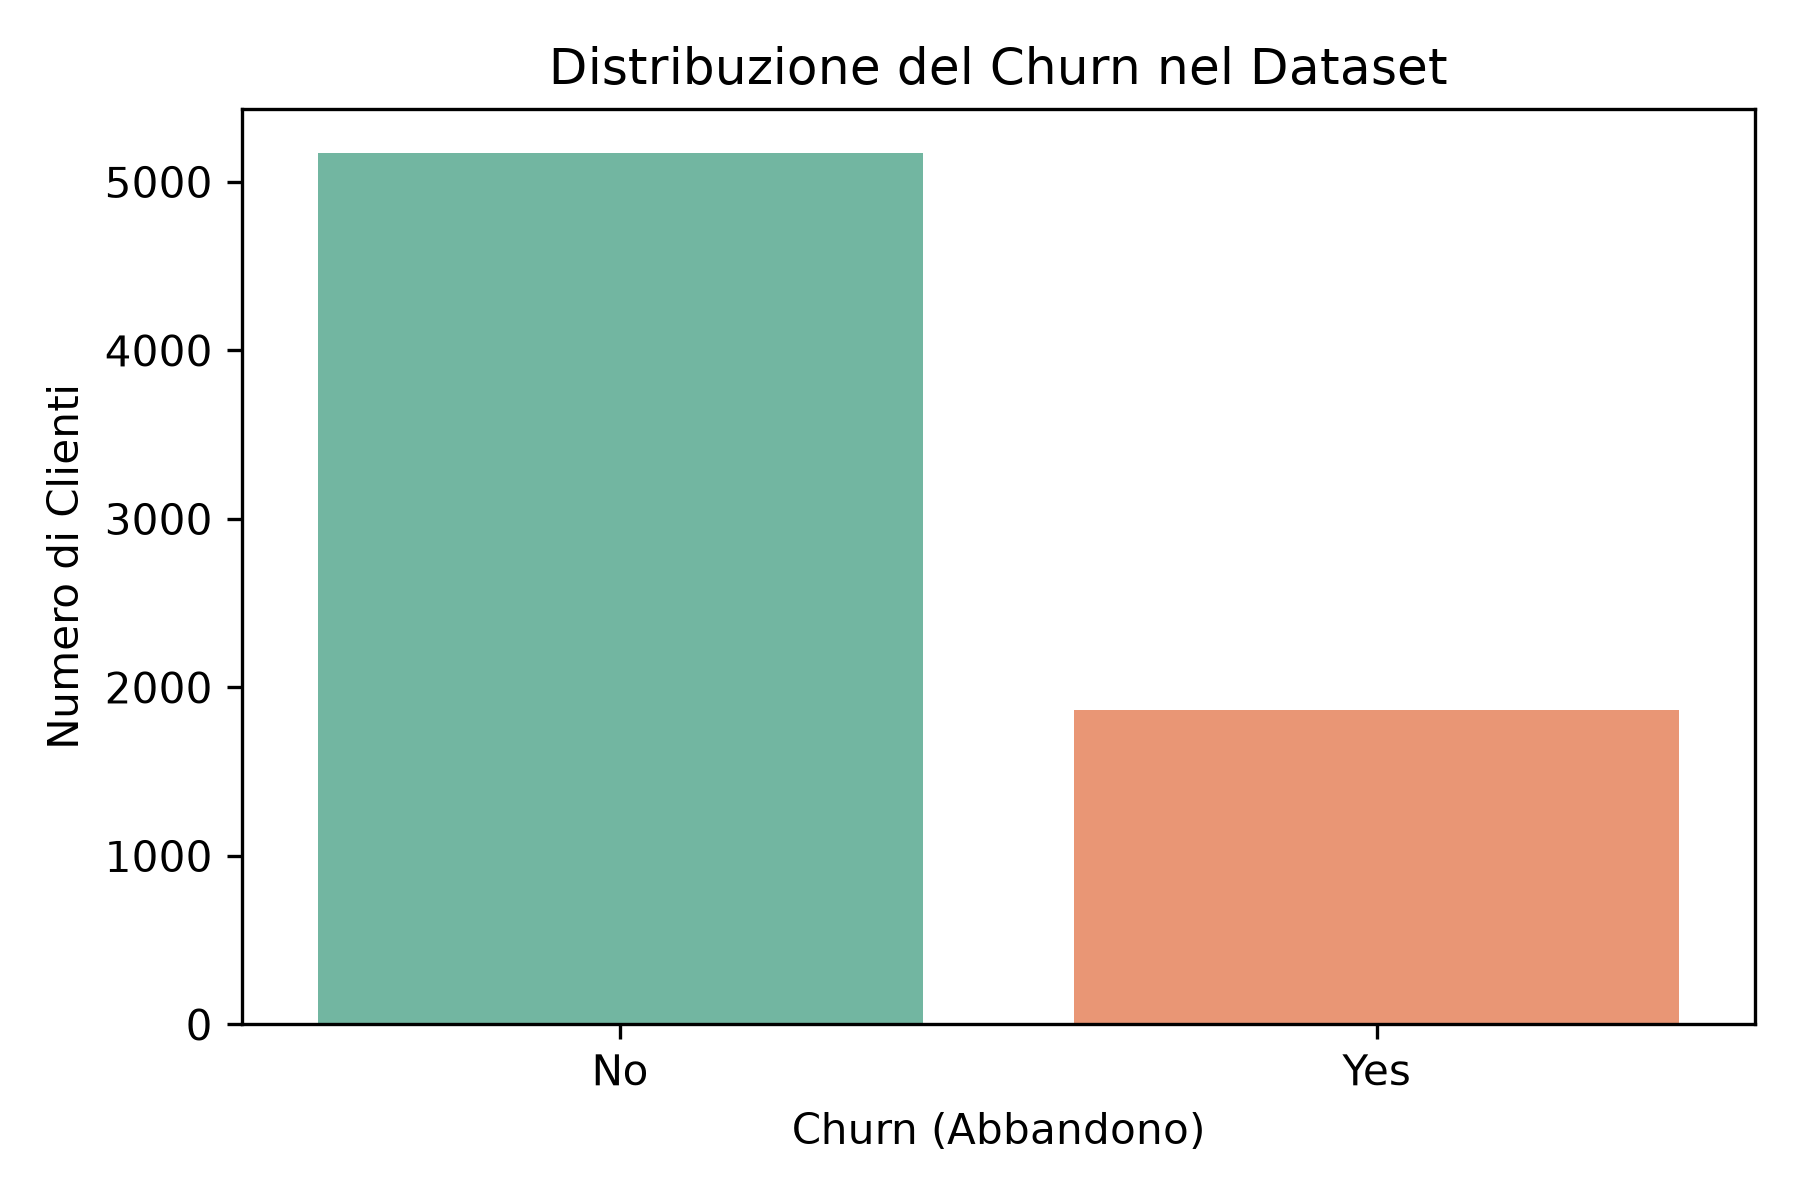
\includegraphics[width=\textwidth]{../grafici/churn_distribution.png}
        \caption{Distribuzione del Churn nel dataset.}
        \label{fig:churn_dist}
    \end{minipage}\hfill
    \begin{minipage}{0.48\textwidth}
        \centering
        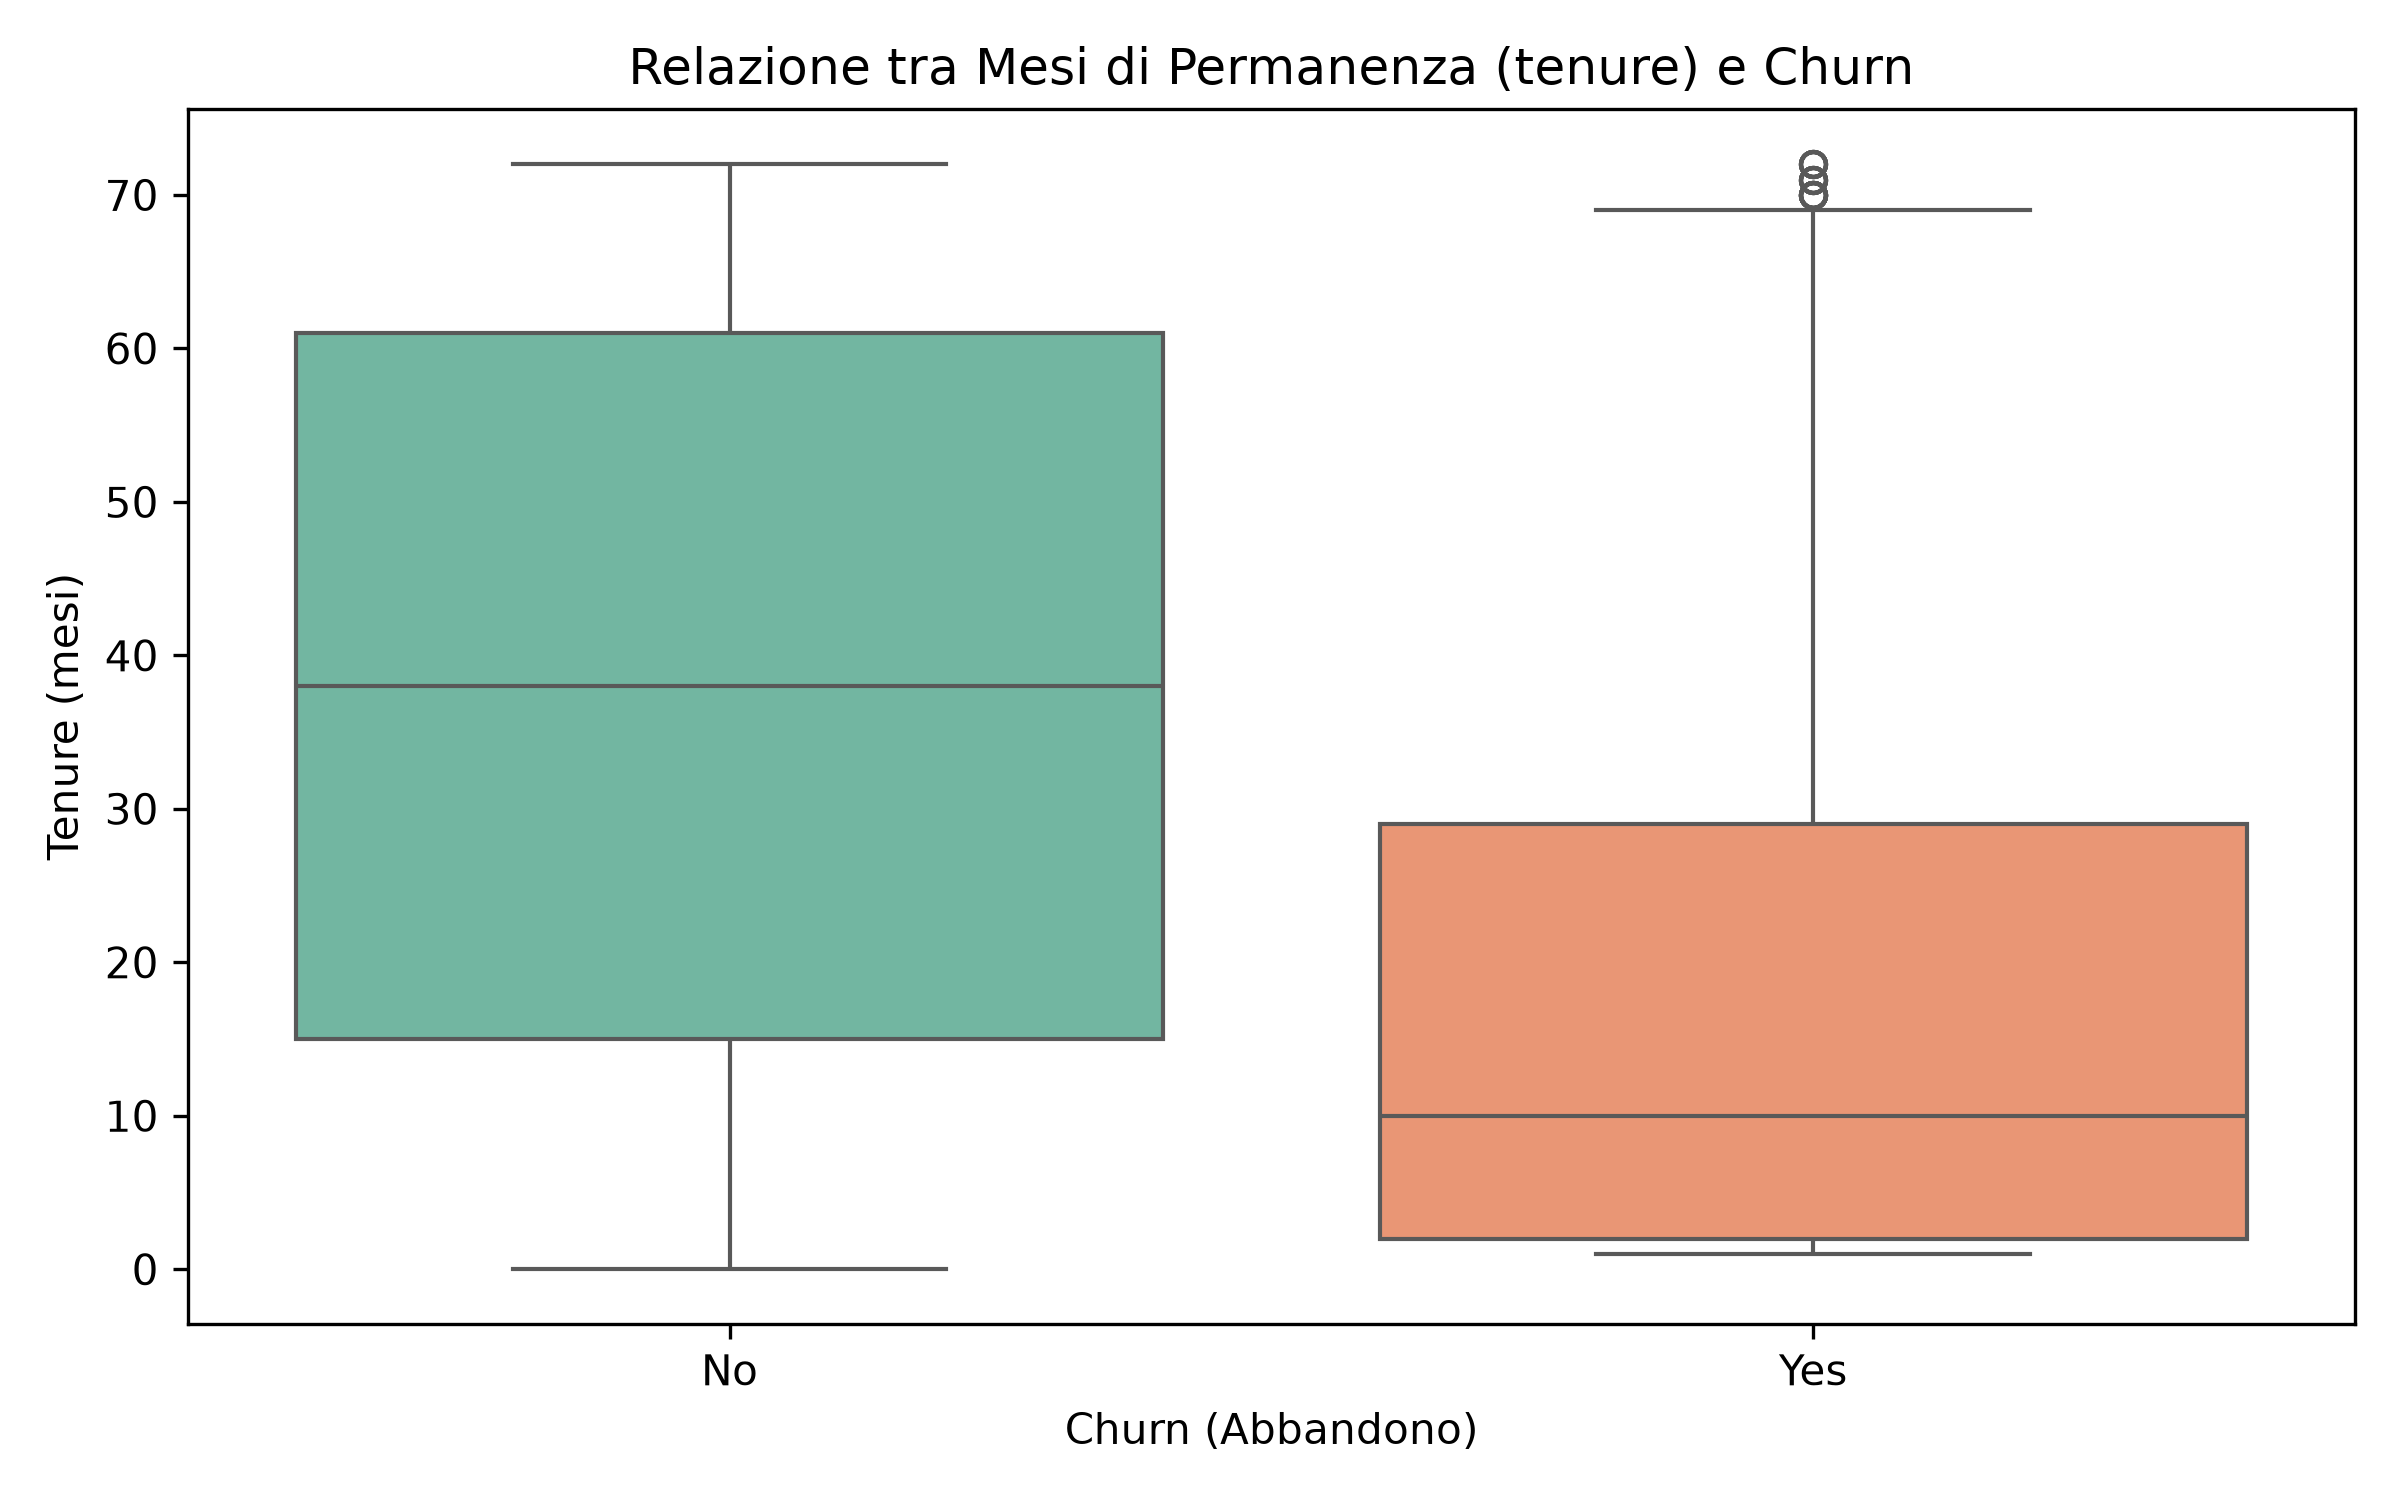
\includegraphics[width=\textwidth]{../grafici/churn_vs_tenure.png}
        \caption{Relazione tra mesi di permanenza (tenure) e Churn.}
        \label{fig:churn_tenure}
    \end{minipage}
\end{figure}

\subsection{Criticità: Sbilanciamento delle Classi}
Il dataset è molto sbilanciato: il $73.4\%$ dei clienti non ha abbandonato (classe $0$), mentre solo il $26.6\%$ ha abbandonato (classe $1$). C'è un rapporto di circa 3 a 1. Se non si fa attenzione, un modello potrebbe limitarsi a dire sempre ``No Churn'' e ottenere un'accuratezza del $73.4\%$ senza capire nulla del problema. Per questo ho eseguito uno split train-test stratificato, per mantenere la stessa proporzione di clienti a rischio sia nel set di addestramento che in quello di test.

% -------------------------------------------------------------
\section{Metodologia}
\label{sec:metodologia}
La mia pipeline di lavoro è divisa in tre parti:
1. Pulizia dei dati, codifica delle categoriche e standardizzazione.
2. Applicazione di $k$-Means per generare la feature del cluster e aggiunta di questa colonna al dataset.
3. Addestramento dei tre classificatori (Regressione Logistica, Albero di Decisione, MLP) sia con che senza la colonna del cluster, per valutarne l'effetto.

\subsection{I Modelli Scelti}

\subsubsection{k-Means (Clustering)}
L'algoritmo $k$-Means serve a dividere i dati in gruppi. All'inizio sceglie a caso dei punti centrali (centroidi) per ogni gruppo. Poi ripete due passi:
\begin{enumerate}
    \item Assegna ogni cliente al gruppo il cui centroide è più vicino (usando la distanza euclidea).
    \item Ricalcola il centro di ogni gruppo facendo la media delle posizioni dei punti assegnati ad esso.
\end{enumerate}
Si ferma quando i centri non si muovono più. Ho provato soluzioni con 2, 3 e 4 cluster valutando Inertia e Silhouette Score per scegliere il numero ottimale di gruppi.

\subsubsection{Regressione Logistica (Baseline)}
Usata come baseline semplice. Calcola una somma pesata delle caratteristiche del cliente e la passa dentro la funzione sigmoide:
\begin{equation}
    \sigma(t) = \frac{1}{1 + e^{-t}}
\end{equation}
Questa funzione schiaccia il risultato in un valore tra 0 e 1, che rappresenta la probabilità che il cliente abbandoni.

\subsubsection{Decision Tree (Modello Principale 1)}
Questo modello ragiona a domande sì/no (regole). Sceglie le suddivisioni migliori per separare il più possibile i clienti a rischio da quelli fedeli, misurando la purità dei gruppi tramite l'indice di Gini. Ho impostato la profondità massima dell'albero a $5$ (\texttt{max\_depth=5}) per evitare che cresca troppo e impari a memoria le risposte (overfitting).

\subsubsection{Multi-Layer Perceptron (Modello Principale 2)}
Il Multi-Layer Perceptron (MLP) è una rete neurale artificiale composta da vari strati di neuroni collegati tra loro.

L'addestramento funziona in due fasi ripetute iterativamente:
\begin{enumerate}
    \item \textbf{Fase in avanti (Forward Propagation)}: I dati del cliente entrano nella rete, passano per gli strati nascosti (dove i neuroni calcolano somme pesate e applicano una funzione di attivazione non lineare come la ReLU, $f(x) = \max(0, x)$) e arrivano all'uscita.
    \item \textbf{Fase all'indietro (Backpropagation)}: Si calcola l'errore tra la risposta della rete e quella reale (usando la perdita di cross-entropia). L'errore viene propagato a ritroso per correggere i pesi dei collegamenti usando un ottimizzatore (Adam) basato sulla discesa del gradiente.
\end{enumerate}

\textbf{Perché nei neuroni nascosti servono funzioni non lineari?}\\
Senza di esse, la composizione di più strati lineari collasserebbe matematicamente in una singola trasformazione lineare. La rete neurale perderebbe così la capacità di apprendere relazioni complesse, diventando equivalente ad un semplice modello di Regressione Logistica.

\textbf{Perché nell'ultimo neurone serve la Sigmoide?}\\
Perché vogliamo che l'output sia una probabilità compresa tra 0 e 1. Se non la usassimo, la rete darebbe in uscita un numero reale qualsiasi, rendendo impossibile interpretarlo come probabilità e calcolare l'errore con la cross-entropia standard per la classificazione binaria.

\subsection{Riproducibilità, Dipendenze e Istruzioni d'Esecuzione}
Per rendere il progetto riproducibile, tutto il codice è racchiuso nel notebook \texttt{segmentazione\_crunch.ipynb}. Se il dataset non è presente localmente nella cartella \texttt{dati/}, il notebook lo scarica da solo all'avvio.

Le librerie usate con le rispettive versioni di riferimento sono:
\begin{itemize}
    \item \textbf{Pandas} e \textbf{NumPy} per gestire le tabelle e i calcoli matematici.
    \item \textbf{Scikit-Learn} per il clustering ($k$-Means) e i modelli di classificazione.
    \item \textbf{Matplotlib} e \textbf{Seaborn} per disegnare i grafici.
\end{itemize}
Le dipendenze esatte sono raccolte nel file \texttt{requirements.txt} e le istruzioni di installazione sono spiegate nel file \texttt{README.md} nella radice del progetto.

% -------------------------------------------------------------
\section{Esperimenti}
\label{sec:esperimenti}

\subsection{Setup Sperimentale e Prevenzione dell'Overfitting}
Per verificare che i modelli funzionino bene su dati nuovi, dobbiamo controllare due problemi:
\begin{itemize}
    \item \textbf{Overfitting (imparare a memoria)}: succede quando il modello si adatta troppo bene ai dati di addestramento (compreso il rumore e i dettagli inutili), ma poi fa molti errori sui dati nuovi del Test Set.
    \item \textbf{Underfitting (troppo semplice)}: succede quando il modello è troppo semplice e non riesce a capire le regole del problema, ottenendo risultati scarsi sia sul Train e sul Test.
\end{itemize}
Per verificare questi comportamenti, ho addestrato i modelli sull'80\% dei dati (Train) e poi li ho valutati sul restante 20\% (Test), confrontando le metriche ottenute nei due casi per essere sicuro che le prestazioni fossero stabili.

\subsection{Caratterizzazione dei due Cluster ($k=2$)}
Dopo aver eseguito l'algoritmo k-Means con $k=2$, ho analizzato le caratteristiche dei clienti nei due gruppi (usando i valori originali prima della standardizzazione):
\begin{enumerate}
    \item \textbf{Cluster 0 (1526 clienti - ``Fedeli e con spesa bassa'')}:
    \begin{itemize}
        \item Tenure media: $30.55$ mesi.
        \item Spesa mensile media (\textit{MonthlyCharges}): $21.08\$$.
        \item Costo totale medio (\textit{TotalCharges}): $662.60\$$.
        \item Tasso di Churn reale: \textbf{7.40\%} (estremamente basso).
        \item Contratti: Prevalenza di contratti a lungo termine (Biennali: $41.8\%$, Annuali: $23.9\%$, Mensili: $34.3\%$).
        \item \textit{Profilo}: Clientela stabile che utilizza servizi di base, caratterizzata da elevata fedeltà e contratti pluriennali.
    \end{itemize}
    \item \textbf{Cluster 1 (5517 clienti - ``A rischio e con spesa alta'')}:
    \begin{itemize}
        \item Tenure media: $32.88$ mesi.
        \item Spesa mensile media (\textit{MonthlyCharges}): $76.84\$$.
        \item Costo totale medio (\textit{TotalCharges}): $2727.03\$$.
        \item Tasso di Churn reale: \textbf{31.83\%} (molto alto).
        \item Contratti: Forte prevalenza di contratti flessibili mensili (Mese-a-mese: $60.7\%$).
        \item \textit{Profilo}: Clientela ad alto consumo tecnologico (banda larga, streaming), ma molto volatile e legata a contratti mensili senza vincoli temporali.
    \end{itemize}
\end{enumerate}

% -------------------------------------------------------------
\section{Risultati}
\label{sec:risultati}

\subsection{Risultati del Clustering k-Means}
Ho testato k-Means con 2, 3 e 4 cluster. I risultati di Inertia e Silhouette Score sono riportati nella Tabella \ref{tab:clustering_metrics}.

\begin{table}[H]
\centering
\caption{Metriche di valutazione del clustering k-Means.}
\label{tab:clustering_metrics}
\begin{tabular}{ccc}
\toprule
\textbf{Numero di Cluster ($k$)} & \textbf{Inertia} & \textbf{Silhouette Score} \\
\midrule
2 & 41817.82 & 0.2946 \\
3 & 30802.81 & 0.2861 \\
4 & 28228.08 & 0.2279 \\
\bottomrule
\end{tabular}
\end{table}

La silhouette score migliore si ottiene con $k=2$ ($0.2946$). Con $k=3$ scende leggermente a $0.2861$, e con $k=4$ cala ancora a $0.2279$. Per questo ho scelto $k=2$ come suddivisione ottimale dei clienti.
La Figura \ref{fig:clustering_eval} mostra l'andamento delle due metriche.

\begin{figure}[H]
    \centering
    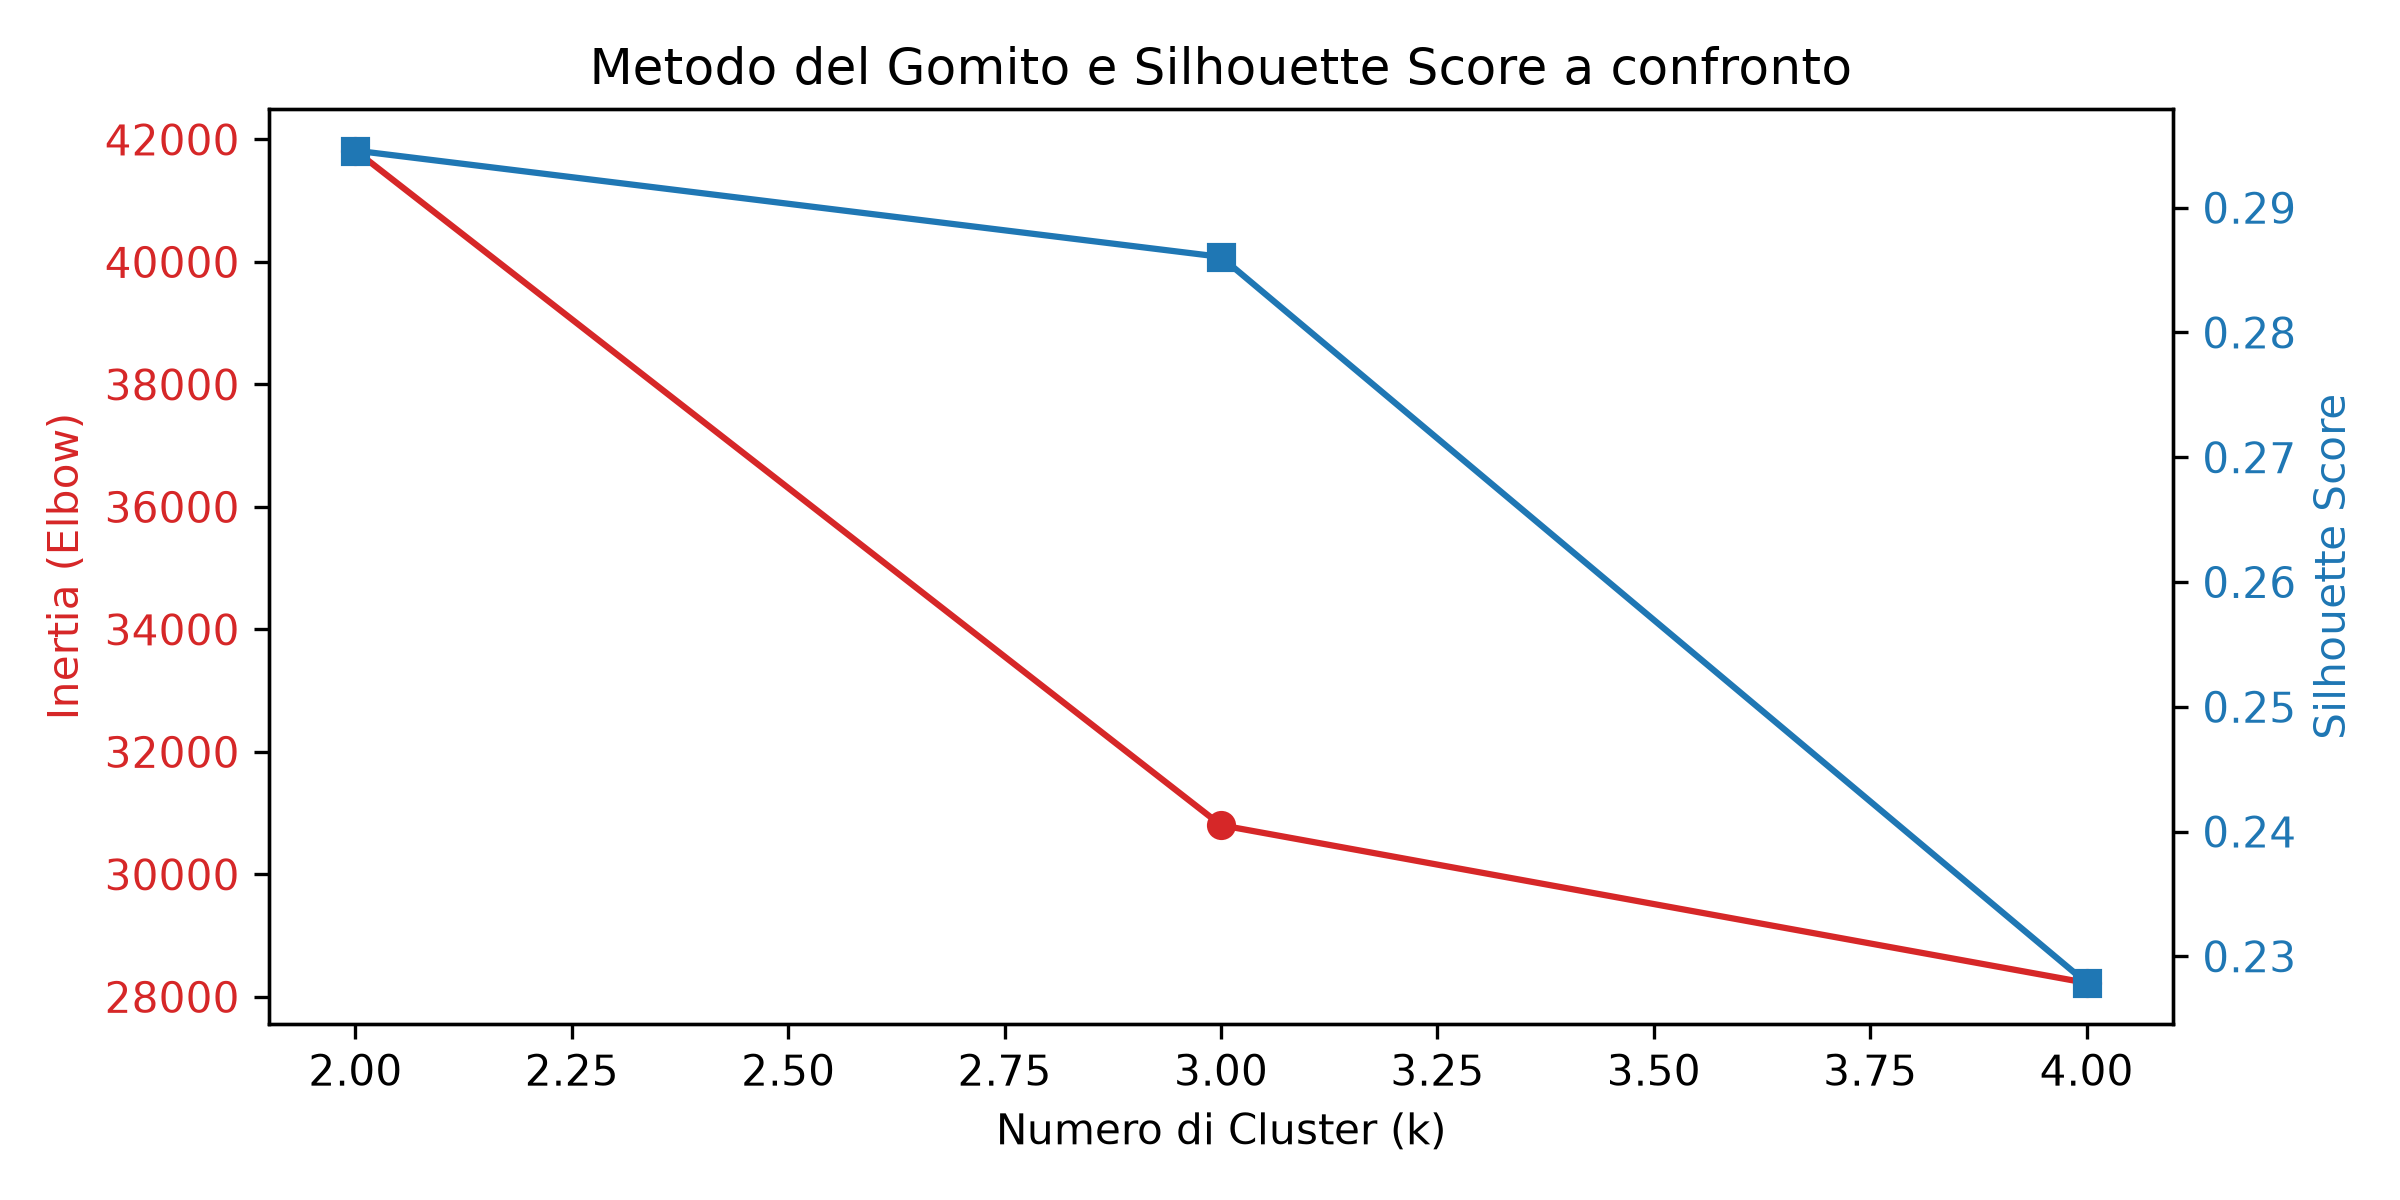
\includegraphics[width=0.85\textwidth]{../grafici/clustering_evaluation.png}
    \caption{Valutazione del clustering k-Means tramite metodo del gomito (Inertia) e Silhouette Score.}
    \label{fig:clustering_eval}
\end{figure}

\subsection{Risultati della Classificazione (Train vs. Test)}
Ho confrontato le prestazioni nei due scenari:
\begin{itemize}
    \item \textbf{Scenario A (Senza Cluster)}: usando solo le caratteristiche originali.
    \item \textbf{Scenario B (Con Cluster)}: aggiungendo il cluster di appartenenza come caratteristica in più.
\end{itemize}
La Tabella \ref{tab:classification_results} riassume le performance di tutti i modelli su Train e Test.

\begin{table}[H]
\centering
\caption{Confronto delle metriche di classificazione tra Train e Test.}
\label{tab:classification_results}
\resizebox{\textwidth}{!}{
\begin{tabular}{llcccccc}
\toprule
 & & \multicolumn{2}{c}{\textbf{Accuracy}} & \multicolumn{2}{c}{\textbf{Recall}} & \multicolumn{2}{c}{\textbf{AUC}} \\
\cmidrule(lr){3-4} \cmidrule(lr){5-6} \cmidrule(lr){7-8}
\textbf{Modello} & \textbf{Feature Scenario} & \textbf{Train} & \textbf{Test} & \textbf{Train} & \textbf{Test} & \textbf{Train} & \textbf{Test} \\
\midrule
Logistic Regression & Senza Cluster & 0.8053 & 0.8062 & 0.5485 & 0.5588 & 0.8492 & 0.8422 \\
Logistic Regression & Con Cluster & 0.8051 & 0.8055 & 0.5485 & 0.5588 & 0.8492 & 0.8423 \\
\midrule
Decision Tree & Senza Cluster & 0.8023 & 0.7942 & 0.5612 & 0.5401 & 0.8476 & 0.8267 \\
Decision Tree & Con Cluster & 0.8023 & 0.7942 & 0.5612 & 0.5401 & 0.8476 & 0.8267 \\
\midrule
Multi-Layer Perceptron (MLP) & Senza Cluster & 0.9143 & 0.7495 & 0.7813 & 0.4278 & 0.9656 & 0.7844 \\
Multi-Layer Perceptron (MLP) & Con Cluster & 0.9104 & 0.7360 & 0.9097 & 0.5829 & 0.9722 & 0.7846 \\
\bottomrule
\end{tabular}
}
\end{table}

\subsection{Analisi dei Risultati e dell'Overfitting}
Dall'ispezione della Tabella \ref{tab:classification_results} emergono tre osservazioni importanti:
\begin{enumerate}
    \item \textbf{Regressione Logistica e Albero di Decisione sono stabili}: Le prestazioni su Train e Test sono quasi identiche (es. accuratezza intorno all'80\% per entrambi). Non c'è alcun segno di overfitting. L'albero di decisione funziona bene perché limitando la profondità massima a 5 gli abbiamo impedito di crescere troppo e memorizzare i dati di addestramento. In questi due modelli l'aggiunta del cluster non cambia i risultati, perché la divisione fatta dal clustering è lineare ed è già contenuta nelle altre variabili originali.
    \item \textbf{La Rete Neurale (MLP) soffre di forte overfitting}: Sul Train set senza cluster l'MLP raggiunge risultati altissimi (Accuratezza $91.43\%$, AUC $0.9656$), ma sul Test set crolla vistosamente (Accuratezza $74.95\%$, Recall $42.78\%$, AUC $0.7844$). Essendo un modello molto complesso con molti parametri, tende a memorizzare i dettagli e il rumore del Train set invece di capire le regole generali.
    \item \textbf{L'impatto del Cluster sull'MLP}: Pur non risolvendo l'overfitting, l'aggiunta del cluster come caratteristica nello Scenario B fa fare un grande balzo in avanti alla \textbf{Recall sul Test set, che sale dal $42.78\%$ al $58.29\%$ ($+15.51\%$ assoluto)}. Questo significa che il cluster aiuta la rete neurale a individuare molti più clienti a rischio di abbandono reale, anche se a costo di qualche falso positivo in più (l'accuratezza sul test scende leggermente al $73.60\%$).
\end{enumerate}

\begin{figure}[H]
    \centering
    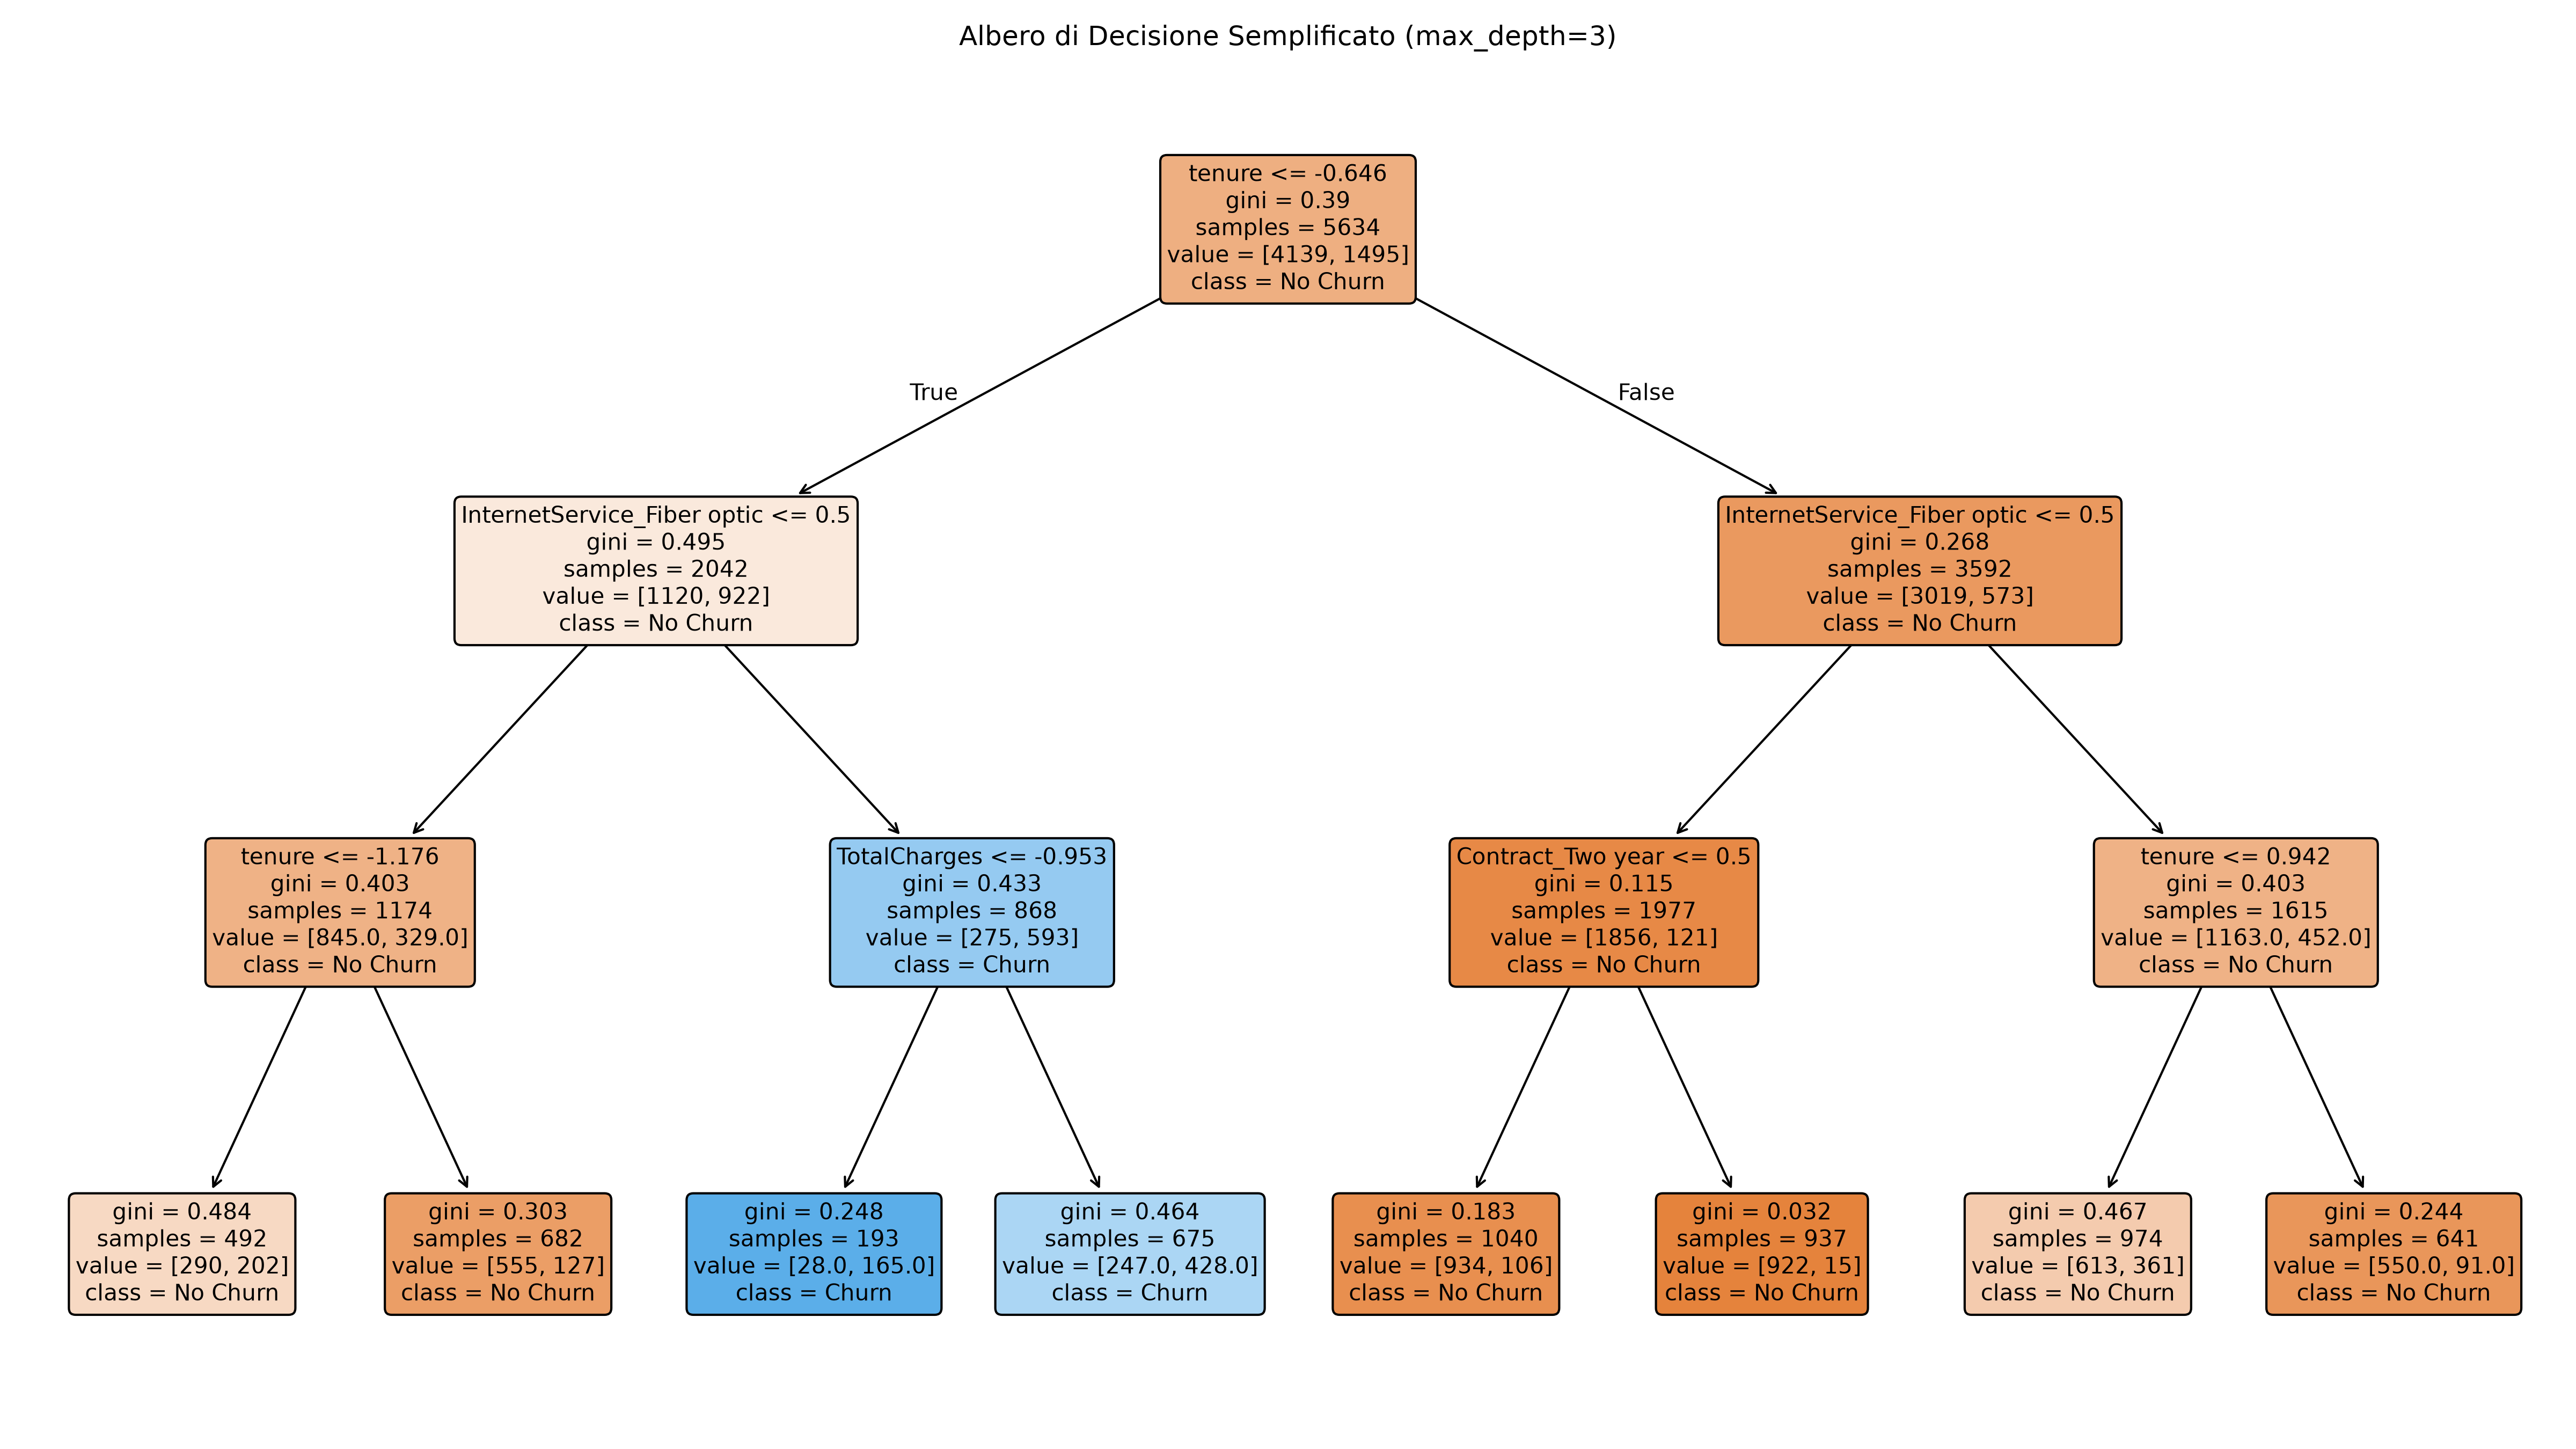
\includegraphics[width=0.9\textwidth]{../grafici/decision_tree_vis.png}
    \caption{Albero di Decisione semplificato (max\_depth=3).}
    \label{fig:decision_tree_vis}
\end{figure}

\begin{figure}[H]
    \centering
    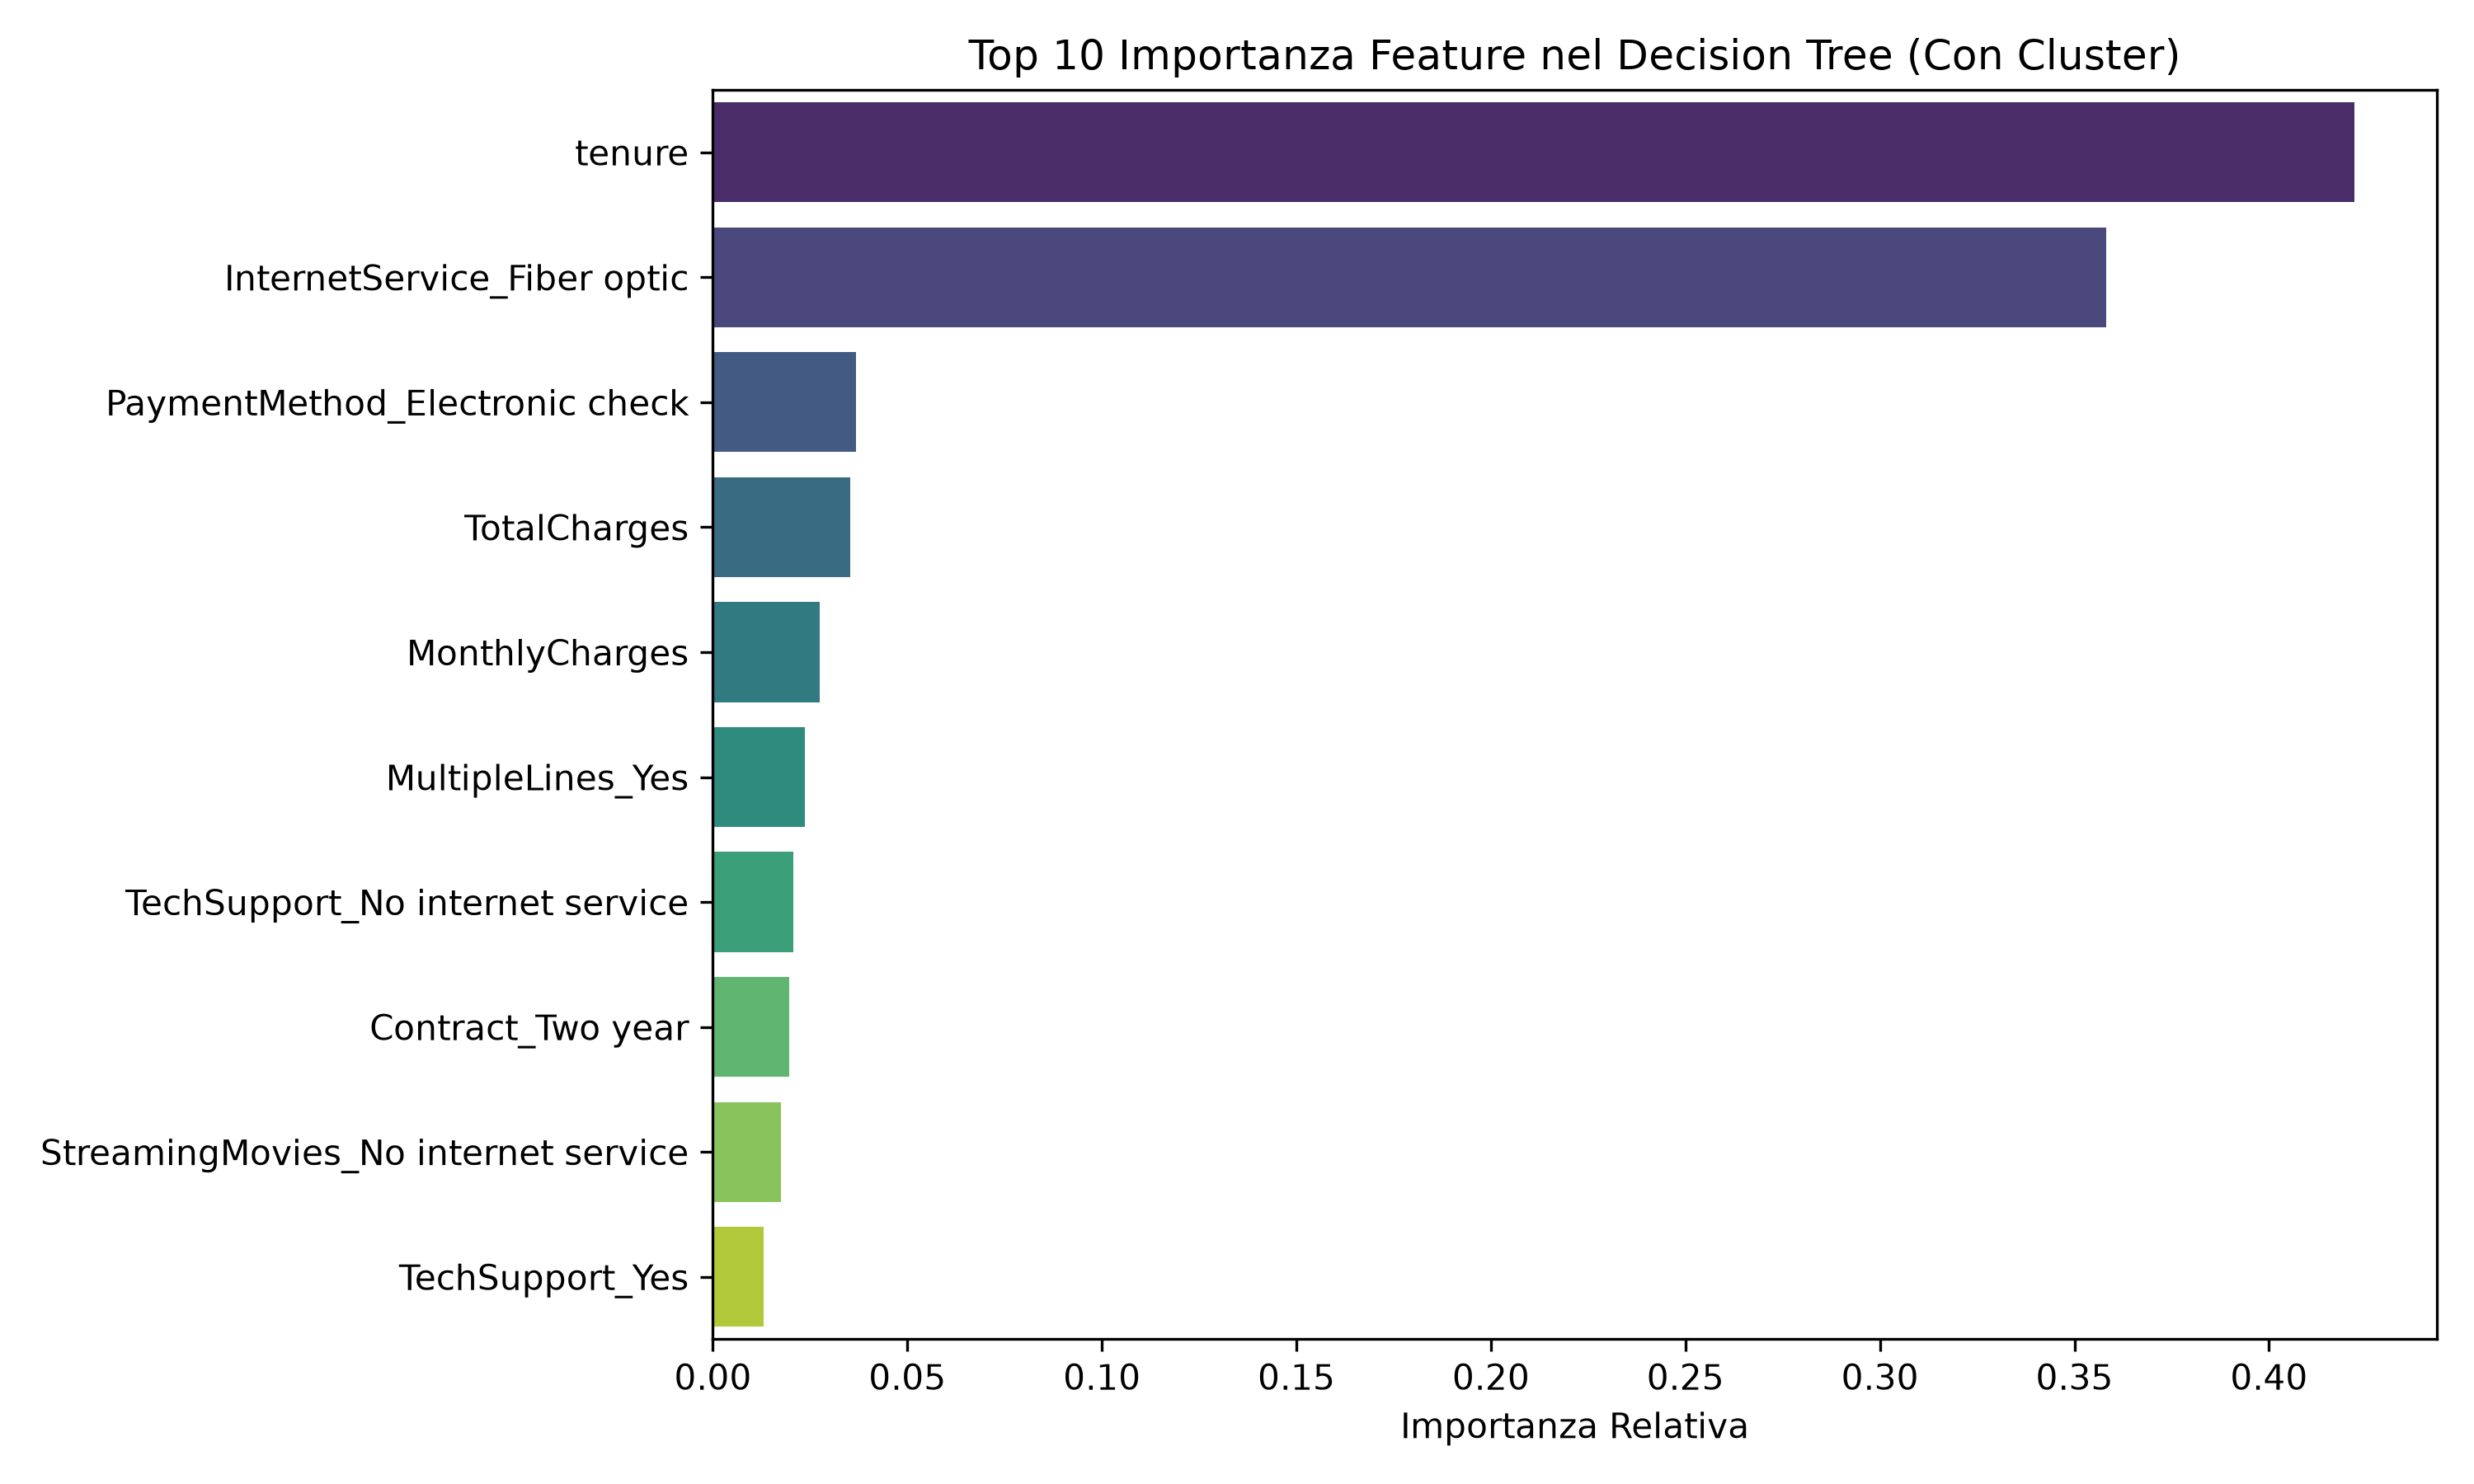
\includegraphics[width=0.8\textwidth]{../grafici/feature_importances.png}
    \caption{Top 10 importanza delle feature per il Decision Tree nello Scenario B (con feature del cluster).}
    \label{fig:feature_importances}
\end{figure}

% -------------------------------------------------------------
\section{Discussione critica}
\label{sec:discussione_critica}

\subsection{Punti di Forza della Soluzione}
Unire il clustering non supervisionato e la classificazione ha permesso di descrivere chiaramente i profili commerciali dei clienti. Inoltre, l'aggiunta del cluster come caratteristica ha dato un aiuto concreto alla rete neurale MLP, aumentandone la Recall sul test set di oltre il $15\%$, un risultato molto utile per l'azienda.

\subsection{Limiti Sperimentali e Fonti di Errore}
I due cluster trovati hanno confini un po' sfumati (Silhouette Score di $0.2946$), segno che i clienti non sono divisi in categorie nette ma hanno comportamenti intermedi. Inoltre, il forte overfitting dell'MLP dimostra che la rete neurale così com'è non è pronta per essere usata, e servirebbero tecniche per frenare questa tendenza (come l'aumento della regolarizzazione L2, il dropout o l'Early Stopping).

\subsection{Confronto: Decision Tree vs. MLP}
L'Albero di Decisione è un modello trasparente (\textit{white-box}): guardando la Figura \ref{fig:decision_tree_vis} si capiscono al volo le regole usate per classificare un cliente (la regola più importante è se il contratto è mensile e quanti mesi di permanenza ha il cliente). La Rete Neurale (MLP), invece, è una scatola nera (\textit{black-box}): anche se offre una Recall migliore, è impossibile spiegare a parole come i pesi dei collegamenti arrivino a quella decisione, rendendola difficile da usare se l'azienda vuole capire i motivi precisi dietro le scelte dei clienti.

\subsection{Miglioramenti Futuri}
Per migliorare i modelli proporrei di:
\begin{itemize}
    \item Usare tecniche come SMOTE (generazione di dati sintetici della classe minoritaria) o pesare di più la classe minore durante l'addestramento per bilanciare i dati.
    \item Provare modelli ensemble come Random Forest o XGBoost, che spesso gestiscono meglio l'overfitting rispetto alle reti neurali su dati tabellari.
\end{itemize}

\subsection{Uso di strumenti di Intelligenza Artificiale Generativa}
Per lo sviluppo di questo progetto ho utilizzato strumenti di intelligenza artificiale generativa (Large Language Models) solo per farmi aiutare a formattare il codice in \LaTeX\ e a impostare lo scheletro della relazione.

\section{Conclusioni}
\label{sec:conclusioni}
Il progetto ha dimostrato che unire apprendimento non supervisionato e supervisionato è una scelta vincente. Il clustering ha identificato due gruppi commerciali chiari (clienti fedeli che spendono poco contro clienti volatili che spendono molto). Aggiungere questa suddivisione come caratteristica ha aiutato a ridurre l'impatto dello sbilanciamento del dataset sulla Rete Neurale (MLP), portando a un incremento del $+15.5\%$ nel richiamo dei clienti a rischio di abbandono sul Test Set, anche se rimangono aperti i problemi di overfitting della rete che richiederanno modelli più regolarizzati in futuro.

\end{document}
